%15 min preso!
\documentclass[xcolor=table,aspectratio=169]{beamer}
\usepackage{beamerthemesplit}
\usepackage{wrapfig}
\usetheme{SPbGU}
\usepackage{pdfpages}
\usepackage{amsmath}
\usepackage{cmap}
\usepackage[T2A]{fontenc}
\usepackage[utf8]{inputenc}
\usepackage[english]{babel}
\usepackage{indentfirst}
\usepackage{amsmath}
\usepackage{tikz}
\usepackage{multirow}
\usepackage[noend]{algpseudocode}
\usepackage{algorithm}
\usepackage{algorithmicx}
\usepackage{fancyvrb}
\usepackage{hyperref} 
\definecolor{links}{HTML}{2A1B81}
\hypersetup{colorlinks,linkcolor=,urlcolor=links}
\usetikzlibrary{calc}
\usetikzlibrary{shapes, backgrounds}
\usetikzlibrary{arrows,automata}
\usetikzlibrary{positioning}
\usetikzlibrary{fit}
\usetikzlibrary{shapes.callouts}
\usetikzlibrary{shapes.misc}
\usepackage{xparse}
\usepackage{fontawesome}

\usepackage{etoolbox,refcount}
\usepackage{multicol}

\usepackage{tabularx}
\newcolumntype{Y}{>{\raggedleft\arraybackslash}X}

\renewcommand{\thealgorithm}{}

\newtheorem{mytheorem}{Theorem}
\renewcommand{\thealgorithm}{}

\newcommand{\tikzmark}[1]{\tikz[overlay,remember picture] \node (#1) {};}
\def\Put(#1,#2)#3{\leavevmode\makebox(0,0){\put(#1,#2){#3}}}

\newcommand{\ltz}{$< 1$}

\tikzset{
    state/.style={
           rectangle,
           rounded corners,
           draw=black, very thick,
           minimum height=2em,
           inner sep=2pt,
           text centered,
           },
}

\tikzset{
    invisible/.style={opacity=0,text opacity=0},
    visible on/.style={alt=#1{}{invisible}},
    alt/.code args={<#1>#2#3}{%
      \alt<#1>{\pgfkeysalso{#2}}{\pgfkeysalso{#3}} % \pgfkeysalso doesn't change the path
    },
}

\tikzset{cross/.style={cross out, draw=black, minimum size=2*(#1-\pgflinewidth), inner sep=0pt, outer sep=0pt, ultra thick},
%default radius will be 1pt. 
cross/.default={1pt}}

\NewDocumentCommand{\mycallout}{r<> O{opacity=0.8,text opacity=1} m m m}{%
\tikz[remember picture, overlay]\node[align=center, fill=cyan!20, text width=#5cm,
#2,visible on=<#1>, rounded corners,
draw,rectangle callout,anchor=pointer,callout relative pointer={(290:0.5cm)}]
at (#3) {#4};
}

\NewDocumentCommand{\mycalloutR}{r<> O{opacity=0.8,text opacity=1} m m m}{%
\tikz[remember picture, overlay]\node[align=center, fill=cyan!20, text width=#5cm,
#2,visible on=<#1>, rounded corners,
draw,rectangle callout,anchor=pointer,callout relative pointer={(30:0.8cm)}]
at (#3) {#4};
}


%callout relative pointer={(230:0.5cm)}]

\newcounter{countitems}
\newcounter{nextitemizecount}
\newcommand{\setupcountitems}{%
  \stepcounter{nextitemizecount}%
  \setcounter{countitems}{0}%
  \preto\item{\stepcounter{countitems}}%
}
\makeatletter
\newcommand{\computecountitems}{%
  \edef\@currentlabel{\number\c@countitems}%
  \label{countitems@\number\numexpr\value{nextitemizecount}-1\relax}%
}
\newcommand{\nextitemizecount}{%
  \getrefnumber{countitems@\number\c@nextitemizecount}%
}
\newcommand{\previtemizecount}{%
  \getrefnumber{countitems@\number\numexpr\value{nextitemizecount}-1\relax}%
}
\makeatother    
\newenvironment{AutoMultiColItemize}{%
\ifnumcomp{\nextitemizecount}{>}{3}{\begin{multicols}{2}}{}%
\setupcountitems\begin{itemize}}%
{\end{itemize}%
\unskip\computecountitems\ifnumcomp{\previtemizecount}{>}{3}{\end{multicols}}{}}


\beamertemplatenavigationsymbolsempty

\title[Графы и линейная алгебра на RISC-V]{Анализ графов и разреженная линейная алгебра в инфраструктуре RISC-V}
\subtitle{Рабочая группа ``Развитие экосистемы ПО на RISC-V''}
\institute[СПбГУ]{
Санкт-Петербургский Государственный Университет
}

% То, что в квадратных скобках, отображается в левом нижнем углу.
\author[Семён Григорьев]{Семён Григорьев}

\date{25 апреля 2025}


\begin{document}
{
\begin{frame}[fragile]
  \begin{table}
  \centering
  %
\includegraphics[height=1.5cm]{pictures/SPbGU_Logo.png}
  \begin{tabularx}{\linewidth}{XcX}
    %
\includegraphics[height=0.9cm]{pictures/hu_logo.jpeg} 
    \hfill
    & 
    & \hfill 
\includegraphics[height=1.6cm]{pictures/SPbGU_Logo.png}
  \end{tabularx}
  \end{table}
  \titlepage
\end{frame}
}

\begin{frame}[fragile]
  \frametitle{Семён Григорьев}
  \begin{minipage}{0.70\textwidth}
  \begin{itemize}    
    \item Доцент кафедры системного программирования Санкт-Петербургского Государственного Университета
    \item Научный сотрудник лаборатории YADRO
    \item Руководитель исследовательской группы
    \item Области интересов
    \begin{itemize}
      \item \textbf{Высокопроизводительная линейная алгебра} для анализа графов
      \begin{itemize}
        \item \textbf{Обобщённая}: матрицы и вектора параметризованы типом элемента, операции над ними могут быть заданы пользователем
        \item \textbf{Разреженная}: специализированные структуры для хранения матриц и векторов, специализированные алгоритмы для их обработки 
        \item В том числе, с использованием \textbf{графических ускорителей}
      \end{itemize}
      \item \textbf{Высокопроизводительный анализ графов}      
    \end{itemize}
    \end{itemize}
\end{minipage}
\begin{minipage}[t]{0.29\textwidth}
  \begin{center}
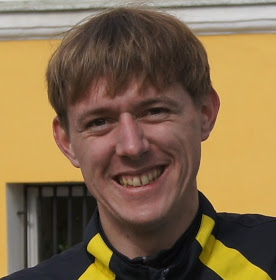
\includegraphics[width=0.8\textwidth]{pictures/SemyonGrigorev.jpg}
  \end{center}
  {\scriptsize
\begin{itemize}    
  \item Email: s.v.grigoriev@mail.spbu.ru
  \item GitHub: \href{https://github.com/gsvgit}{gsvgit}
  \item Google Scholar: \href{https://scholar.google.com/citations?hl=ru&user=kP4dqUAAAAAJ&view_op=list_works&sortby=pubdate}{Semyon Grigorev}
  \item DBLP: \href{https://dblp.org/pid/181/9903.html}{Semyon V. Grigorev}
\end{itemize}
  }
\end{minipage}
\end{frame}

\begin{frame}[fragile]
  \frametitle{Алгоритмы анализа графов\footnote{Наше сообщество на GitHub: \url{https://github.com/FormalLanguageConstrainedPathQuerying}}}
  \begin{itemize}
      \item Разработка, реализация и оптимизация алгоритмов
      \item На основе линейной алгебры (GraphBLAS)
      \begin{itemize}
        \item[\faCheck] Разработаны алгоритмы поиска путей с ограничениями в виде формальный языков
        \begin{itemize}
          \item Регулярные языки, Regular Path Querying, RPQ: часть ISO-стандарта языка запросов\footnote{ ISO/IEC 39075:2024 Information technology --- Database languages --- GQL: \url{https://www.iso.org/standard/76120.html}}
          \item Контекстно-свободные языки, ContextFree Path Querying, CFPQ: анализ программ
        \end{itemize}
        \item LAGraph --- основная открытая библиотека алгоритмов на основе GraphBLAS
        \begin{itemize}
          \item[\faCheck] Базовая версия CFPQ\footnote{\url{https://github.com/GraphBLAS/LAGraph/pull/265}}
          \item[\faCheck] Базовая версия RPQ\footnote{\url{https://github.com/GraphBLAS/LAGraph/pull/261}}
          \item[\faGears] Перенести различные вариации алгоритмов CFPQ и RPQ и их оптимизации
        \end{itemize}  
      \end{itemize}
      \item Интеграция алгоритмов
      \begin{itemize}
        \item[\faCheck] В графовые базы данных (RedisGraph, Neo4j)
        \item[\faGears] В инструменты статического анализа
      \end{itemize}
  \end{itemize}
\end{frame}


\begin{frame}[fragile]
  \frametitle{Библиотеки линейной алгебры для анализа графов\footnote{Наше сообщество на GitHub: \url{https://github.com/SparseLinearAlgebra}}}
  \begin{itemize}
    \item Линейная алгебра на GPGPU
    \begin{itemize}
      \item[\faCheck] cuBool\footnote{\url{https://github.com/SparseLinearAlgebra/cuBool}}: разреженная булева линейная алгебра на Cuda
      \item[\faCheck] Spla\footnote{\url{https://github.com/SparseLinearAlgebra/spla}}: обобщённая разреженная линейная алгебра на OpenCL
      \item[\faGears] Перенос Spla на RISC-V
    \end{itemize}
    \item Вклад в экосистему GraphBLAS
    \begin{itemize}
      \item[\faCheck] Векторизация умножения матриц на RISC-V RVV1.0\footnote{Реквест с изменениями: \url{https://github.com/DrTimothyAldenDavis/GraphBLAS/pull/381}} в SuiteSparse:GraphBLAS\footnote{Референсная реализация GraphBLAS}
      \item[\faGears] Кросс-сборка ``стека'' SuiteSparse:GraphBLAS
    \end{itemize}
    \item[\faGears] Эксперименты с RISC-V GPGPU Vortex
  \end{itemize}
\end{frame}

\begin{frame}[fragile]
  \frametitle{Набор данных для экспериментального исследования алгоритмов}
  \begin{itemize}
    \item Данные из различных областей для исследования производительности RPQ и CFPQ
    \begin{itemize}
      \item Анализ семантических сетей
      \item Статический анализ кода
      \item Биоинформатика
      \item \ldots
    \end{itemize}    
    \item[\faCheck] Набор данных\footnote{CFPQ\_Data: \url{https://github.com/FormalLanguageConstrainedPathQuerying/CFPQ_Data}}
    \item[\faGears] Интеграция в SuiteSparse Matrix  Collection 
  \end{itemize}
\end{frame}

%\begin{frame}[fragile]
%  \frametitle{Образование}
%  \begin{itemize}
%    \item Высокопроизводительный анализ графов
%    \begin{itemize}
%      \item На основе линейной алгебры
%      \item Другие подходы и инструменты (Pregel, GunRock)
%    \end{itemize}    
%    \item Расширение курса по теории формальных языков
%      \begin{itemize}
%        \item[\faCheck] Задачи, система проверки\footnote{\url{https://github.com/FormalLanguageConstrainedPathQuerying/formal-lang-course}}
%        \item[\faGears] Разрабатывается конспект лекций\footnote{\url{https://github.com/FormalLanguageConstrainedPathQuerying/FormalLanguageConstrainedReachability-LectureNotes}}
%      \end{itemize}
%  \end{itemize}
%\end{frame}

\begin{frame}[fragile]
  \frametitle{Итого}
  \begin{itemize}
    \item Опыт разработки, реализации, оптимизации высокопроизводительных алгоритмов анализа графов
    \item Активно коммуницируем с международным сообществом вокруг GraphBLAS и графовых баз данных в целом
    \begin{itemize}
      \item Конференции, публикации
      \item Вклад в проекты с открытым исходным кодом
    \end{itemize}
    \item Работаем в экосистеме RISC-V
    \begin{itemize}
      \item Лаборатория на Математико-Механическом факультете
      \item Вклад в проекты с открытым исходным кодом
      \item Образовательная деятельность
    \end{itemize}
  \end{itemize}
\end{frame}

\end{document}
